%% introduction.tex
%%

%% ==============================
\chapter{Introduction}
\label{ch:Introduction}
%% ==============================
    \section{Neutrinos in the standard model}
    \label{ch:Introduction:sec:Neutrinos in the standard model}
    During the second part of the 20th century, a model stating 16 particles has been developed to describe a huge portion of known phenomena, the standard model. It contains six quarks, six leptons (both made up of three particle generations) and four types of Gauge Bosons. The latter are carriers of the standard models interactions of the former particles, meaning all interactions of matter are based on the exchange of one or more of the Gauge Bosons. 
    For our universe, gravity, the graviton generated force, plays a major role for formation and stability af almost all larger structures. In particle physics however, it can mostly be neglected. Here, only the strong and weak as well as the electromagnetic interaction make for noticable contributions to phenomena observed.
    Most of what we can observe with our bare eyes or in basic experiments is attributable to the electromagnetic force or gravity, however, strong and weak interaction do play a major role when it comes to high energy physics. Here, the limited reach of the two is overcome by small distances between interacting particles. In case of the neutrino, detection and by that the study of its characteristics is even more difficult as it interacts only gravitationally and weakly. Now, as mentioned before, gravity is indeed long range, but very weak in force. And although weak intraction is a lot stronger compared to gravity, it is still weak compared to both electromagnetic and strong interactions. That is why the neutrino is considered elusive, detection efficiencies are low and only large scale detectros are able to detect statistically relevant amounts of neutrinos.
    In the standard model, neutrinos are considered massless. 
    Many experiments have shown that the weightless neutrino is a wrong assumption. Most of these were experiments prooving neutrino oscillatinos with both reactor neutrinos and solar neutrinos such as Kamiokande\cite{PhysRevLett.110.181802} or SNO \cite{SNOOscillations} \todo{add experiments}.
    
    Up till now, only the differences of the squared masses are known. This leads to different relations depending on how masses are distributed between the flavours, \ref{fig:massSchemes}, and how large they are absolutely \ref{fig:massHierarchy}. This problem is solved by the knowledge of one of the masses. KATRIN is on the verge of finding the $\nu_e$'s mass.\cite{becker2008a}
    
    \begin{figure}
    \centering
    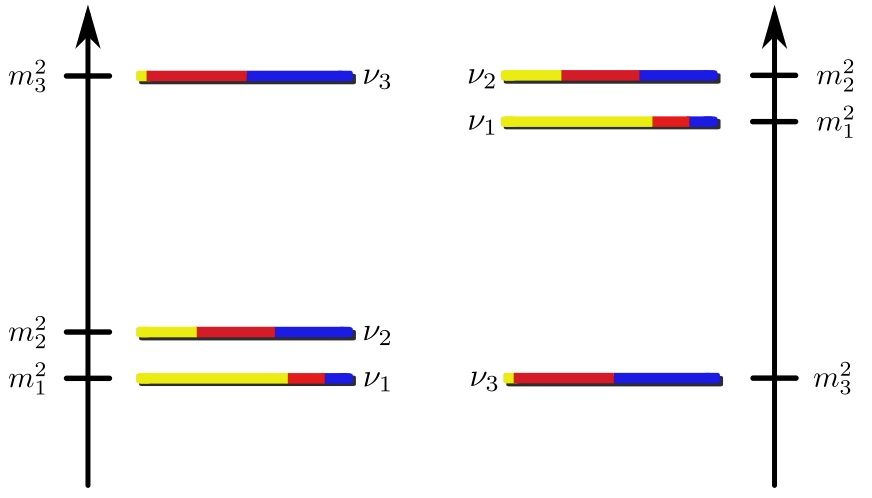
\includegraphics[width=0.5\textwidth]{graphics/standardModel/massHierarchy.jpg}
    	\caption{sadf\cite{neutrinoMassScheme}}
    	\label{fig:massSchemes}
    \end{figure}
    \begin{figure}
    \caption{asdf}
    	\label{fig:massHierarchy}
    \end{figure}

    
    \subsection{Neutrino Oscillations}
    \label{ch:Introduction:sec:Massive neutrino:subsec:neutrino Oscillations}
      If the neutrinos were without mass, its mass eigenstates would equal its flavour eigenstates:
      
    \begin{equation}
	\begin{array}{ccc}
      	|\nu_e>		& = & |\nu_1>\\
      	|\nu_\mu>	& = & |\nu_2>\\
      	|\nu_\tau>	& = & |\nu_3>\\
    	 \end{array}
    \end{equation}
    First doubts concerning this asumptions occured as inconsistencies between the measured and the calculated solar $\nu$-flux occured. As the count on $\nu_e$ was too low, the theory of neutrino oscillations emerged, stating that a mixture of flavours was possible as the flavours were made up of all three of the mass eigenstates. The mixture is described by the so called Pontecorvo-Maki-Nakagawa-Sakata matrix:
        \begin{equation}
        \left(
        \begin{array}{c}
	  |\nu_e>\\
	  |\nu_\mu>\\
	  |\nu_\tau>\\
        \end{array}
        \right)
	 = \left(
	\begin{array}{ccc}
      	\theta_{e,1} & \theta_{e,2} & \theta_{e,3}\\
      	\theta_{\mu,1} & \theta_{\mu,2} & \theta_{\mu,3}\\
      	\theta_{\tau,1} & \theta_{\tau,2} & \theta_{\tau,3}\\
      	\end{array}
	\right)
	\left(
	\begin{array}{c}
      	|\nu_1>\\
      	|\nu_2>\\
      	|\nu_3>\\
    	 \end{array}
    	 \right)
    \end{equation}
    
    \subsection{Direct measurement of neutrino mass}
    \label{ch:Introduction:sec:Massive neutrino:subsec:direct Neutrino Mass measurement}
    Direct measurements of the neutrino mass require a reaction known to include neutrinos in its equation. There are both spectrometric and calorimetric approaches. While the scale of spectrometers is getting bigger and bigger, calorimetric approaches seem to be a reasonable alternative, although the slow detector response - the detector material itself is decaying - requires for large arrays of detectors leading to extensive space requirements as well at some point. The luminosity of spectrometer experiments though is unachieved by any other. That is why the KATRIN collaboration is working on a setup to measure electrons from Tritium decay to determine the neutrino mass. 
     
    \subsection{Indirect measurement of neutrino mass}
    \label{ch:Introduction:sec:Massive neutrino:subsec:indirect Neutrino Mass measurement}
    Another approach is using indirect ways of finding the neutrino mass. One possibility here is to search for neutrinoless double beta decay, $0\nu\beta\beta$, which can exist only if the neutrino is its own anti-particle, a so called majorana neutrino. Then, if two nuclei beta decay, the neutrino from one vertex can be absorbed in the second as an anti-neutrino - or vice versa. The decay would then not emit any neutrino and the rate would be dependant on the "effective Majorana neutrino mass square" \cite{currentNeutrinoSearches}:
    \begin{equation}
    	\Gamma_{0\nu\beta\beta} \propto \left| \sum{U_{ei}^2m\left(\nu_i\right)}\right|^2
    \end{equation}

    
    \section{Cosmic muons and their interaction with matter}
    \label{ch:introduction:sec:Cosmic Air Showers}
    When high energy particles hit the upper parts of the atmosphere, a cascade of particles generated from the interaction with atmospheric molecules and atoms follows. Most primary particles are nucleons, most of which again are free protons, i.e. Hydrogen ions. Helium nucleons' fluxes are already about a order of magnitude below that, higher mass number nuclei show even lower rates\cite{highEnergyCosmicRays}. By different interactions, secondary partcles are created. Any particle satisfying the inequation \begin{equation}
      E_{sec,kin} + m_{sec} c^2 < E_{prim,kin} + m_{prim}
    \end{equation}
    can be created. Mostly pions at first, those cascade further. Often through intermediate photons muons emerge. These travel towards the earths surface often close to the speed of light due to their small masses. Even at these high speeds, the muons' average decay time of around \SI{2.2}{\micro\second} \cite{muonLifetime} is too small for many muons to reach the earth's surface from our reference frame's point of view. In the most common production height of \SI{2}{\kilo\meter} \cite{muonProductionHeight}, the non relativistic time of flight for a \SI{90}{\percent} speed of light particle would be
    \begin{equation}
	t_{class} = \SI{2}{\kilo\meter} / 0.9\cdot c = 
    \end{equation}
    meaning only time dilation from special relativity makes the muon flux as large as ist is:
    \begin{equation}
    	t_{rel} = t_{class} / \sqrt{1-0.9^2}
    \end{equation}
    meaning from our reference frame, the lifetime is prolonged by a factor of around 5, being already enough to reach the surface from heights of \SI{3}{\kilo\meter}. Most muons have even higher energies, making it possible for them to reach surface from greater heigts and under non perpendicular angles towards it.
    For KATRIN, this poses a problem. A smaller flux would be advantageous, as muons may, through different kinds of interaction, cause emission of electrons from the spectrometer vessels surface.


